\subsection{无穷小比阶}

	\begin{ti}
		当 $x \to 0$ ,$(1 - \cos x)\ln\left( 1 + 2x^{3} \right)$ 是比 $x \sin x^{n}$ 高阶的无穷小,而 $x \sin x^{n}$ 是比 $\ee^{x\tan^{2} x} - 1$ 高阶的无穷小,则正整数 $n = $ \htwo.
	\end{ti}

	\begin{ti}
		当 $x \to 0^{+}$ 时,$\sqrt{1 + \tan \sqrt{x}} - \sqrt{1 + \sin\sqrt{x}}$ 是 $x$ 的 $k$ 阶无穷小,则 $k =$ \htwo.
	\end{ti}

	\begin{ti}
		当 $x \to 0$ 时,$f(x) = \ln\left( 1+x^{2} \right) - 2\sqrt[3]{\left( \ee^{x} - 1 \right)^{2}}$ 是无穷小量 $x^{k}$ 的同阶无穷小,则 $k = $ \kuo.

		\fourch{$1$}{$2$}{$\frac{2}{3}$}{$\frac{3}{2}$}
	\end{ti}

	\begin{ti}
		当 $x \to 0$ 时,下列无穷小量中,最高阶的无穷小是\kuo.

		\twoch{$\ln\left( x + \sqrt{1 + x^{2}} \right)$}{$1 - \cos x$}{$\tan x - \sin x$}{$\ee^{x} + \ee^{-x} - 2$}
	\end{ti}

	\begin{ti}
		当 $x \to 0^{+}$ 时,下列无穷小量中,与 $x$ 同阶的无穷小是\kuo.

		\twoch{$\sqrt{1 + x} - 1$}{$\ln(1 + x) - x$}{$\cos(\sin x) - 1$}{$x^{x} - 1$}
	\end{ti}

	\begin{ti}
		当 $x \to 0$ 时,$f(x) = x - \sin x + \int_{0}^{x} t^{2} \ee^{t^{2}} \dd{t}$ 是 $x$ 的 $k$ 阶无穷小,则 $k=$ \kuo.

		\fourch{$3$}{$4$}{$5$}{$6$}
	\end{ti}

	\begin{ti}
		当 $x \to 0^{+}$ 时,试比较无穷小量 $\alpha$,$\beta$ 和 $\gamma$ 三者之间的阶,其中
		\[
			\alpha = \int_{0}^{x} \cos t^{2} \dd{t},\beta = \int_{0}^{x^{2}} \tan \sqrt{t} \dd{t},\gamma = \int_{0}^{\sqrt{x}} \sin t^{3} \dd{t}.
		\]
	\end{ti}

	\begin{ti}
		当 $x \to 0$ 时,$\sin x \left( \cos x - 4 \right) + 3x$ 为 $x$ 的几阶无穷小?
	\end{ti}

	\begin{ti}
		当 $x \to 0$ 时,确定下列无穷小量的阶数:
		\begin{enumerate}
			\item $\tan\left( \sqrt{x+2} - \sqrt{2} \right)$;
			\item $\sqrt[3]{1 + \sqrt[3]{x}} - 1$;
			\item $3^{\sqrt{x}} - 1$.  
		\end{enumerate}
	\end{ti}

	\begin{ti}
		当 $x \to 0$ 时,$x - \sin x \cos x \cos 2x$ 与 $cx^{k}$ 为等价无穷小,则 $c=$ \htwo,$k=$ \htwo.
	\end{ti}

	\begin{ti}
		当 $x \to 0$ 时,$1 - \cos x \cos 2x \cos 3x$ 对于无穷小 $x$ 的阶数等于 \htwo.
	\end{ti}

	\begin{ti}
		极限 $\lim_{x \to \infty} \frac{\ee^{\sin\frac{1}{x}}-1}{\left( 1 + \frac{1}{x} \right)^{\alpha} - \left( 1 + \frac{1}{x} \right)} = A \ne 0$ 的充要条件是
		
		\noindent\kuo.

		\twoch{$\alpha > 1$}{$\alpha \ne 1$}{$\alpha > 0$}{与 $\alpha$ 无关}
	\end{ti}

	\begin{ti}
		设当 $x \to 0$ 时,$\ee^{\tan x} - \ee^{x}$ 与 $x^{n}$ 是同阶无穷小,则 $n$ 为 \kuo.

		\fourch{$1$}{$2$}{$3$}{$4$}
	\end{ti}

	\begin{ti}
		设当 $x \to 0$ 时,$f(x) = ax^{3} + bx$ 与 $g(x) =$ $\int_{0}^{\sin x} \left( \ee^{t^{2}} -1 \right) \dd{t}$ 是等价无穷小,则\kuo.

		\twoch{$a = \frac{1}{3},b=1$}{$a = 3,b=0$}{$a = \frac{1}{3},b=0$}{$a = 1,b=0$}
	\end{ti}

	\begin{ti}
		设当 $x \to 0$ 时,$f(x) = \ln\left( 1+x^{2} \right) - \ln\left( 1 + \sin^{2}x \right)$ 是 $x$ 的 $n$ 阶无穷小,则正整数 $n$ 为\kuo.
		
		\fourch{$1$}{$2$}{$3$}{$4$}
	\end{ti}

	\begin{ti}
		当 $x \to \uppi$ 时,若有 $\sqrt[4]{\sin\frac{x}{2}} - 1 \sim A(x - \uppi)^{k}$,则 $A=$\htwo,$k=$\htwo.
	\end{ti}

	\begin{ti}
		半径分别为 $R,r(R>r>0)$ 的两个圆相切于坐标轴原点. 如图~\ref{fig:1.1.1} 所示.
		\begin{enumerate}
			\item 当 $x \to 0^{+}$ 时,若线段长 $MM_{1}$ 与 $x^{k}$ 同阶,求 $k$;
			\item 当 $x \to 0^{+}$ 时,若 $\angle MOM_{1}$ 与 $x^{c}$ 同阶,求 $c$.
		\end{enumerate}
		\begin{figure}[htbp]
			\centering
			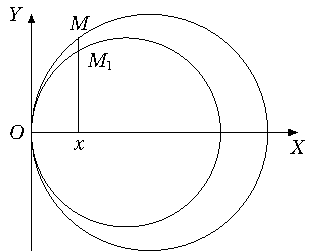
\includegraphics[scale=1]{figure/fig1-1-1.pdf}
			\caption{}\label{fig:1.1.1}
		\end{figure}
	\end{ti}